\chapter{汽化器侧出口堵销}
\begin{figure}[htbp]
\centering
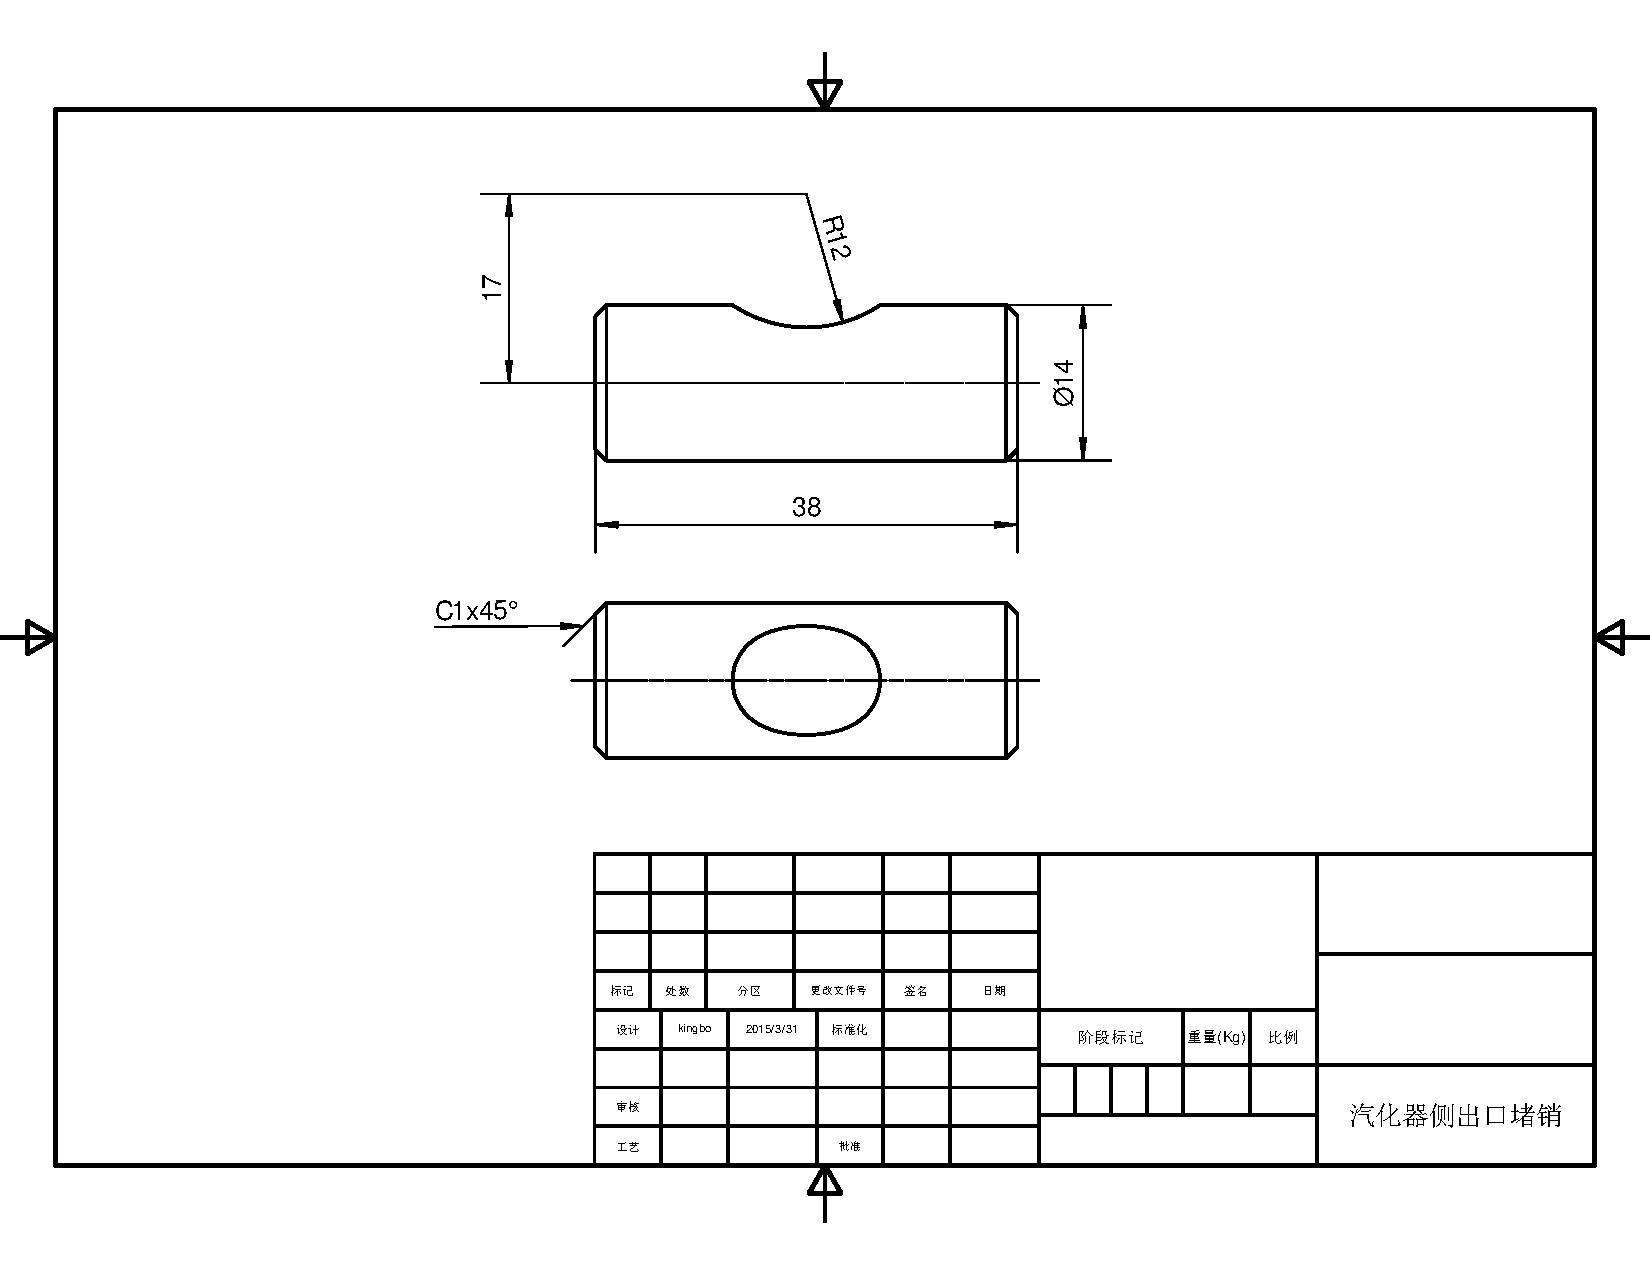
\includegraphics[scale=0.45,angle=-90]{chechukouxiao}
\caption{汽化器侧出口堵销零件图}\label{fig:chechukouxiao}
\end{figure}
%AutoCAD作为国际上广泛使用的流行的绘图工具,它具有较强的二维绘图和三维绘图功能,欢迎来到AutoCAD的三维世界,
本章我们的目标是用AutoCAD制作图\ref{fig:chechukouxiao}所示的航模发动机汽化器侧出口堵销零件的三维模型。本章将学习以下内容:
\begin{itemize}
	\item 截交体的概念
	\item 差集操作
\end{itemize}
\section{汽化器侧出口堵销建模}
\begin{procedure}
\item 切换视图方向

通过观察\ref{fig:chechukouxiao}可知汽化器侧出口堵销零件的表达视图有主视图和俯视图,基于连杆转销的三维建模经验,可知尺寸$\phi 14$清晰地表明了汽化器侧出口堵销零件是轴类零件,其表达其回转体特征的左视图被省略。为例构建的三维模型与主视图方面一致,需要先将视图切换至左视图。

\begin{lstlisting}
命令: -view 
输入选项 [?/删除(D)/正交(O)/恢复(R)/保存(S)/设置(E)/窗口(W)]:left
\end{lstlisting}

完成左视图切换后,$x-y$坐标系已经与左视图投影面平行,为便于观察三维模型的构建过程,需要现次运用视图切换命令将视图切换为西南等轴测,进入三维视图模式。

\begin{lstlisting}
命令: -view 
输入选项 [?/删除(D)/正交(O)/恢复(R)/保存(S)/设置(E)/窗口(W)]:swiso 
\end{lstlisting}

\item 构建堵销基础圆柱体

完成视图切换后,忽略汽化器侧出口堵销零件上的缺口和倒角等细节后,可知视图表达的是一圆柱体,因此调用AutoCAD中的圆柱体命令来构建基础圆柱体。建模结果如图\ref{fig:chechukouduxiaojianmo1}所示。

\begin{figure}[htbp]%
\centering
\begin{floatrow}[2]
\ffigbox{\caption{构建基础圆柱体}\label{fig:chechukouduxiaojianmo1}}{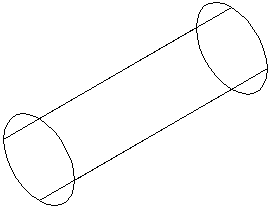
\includegraphics[scale=0.6]{chechukouduxiaojianmo1.png}}
\ffigbox{\caption{添加切除圆柱体}\label{fig:chechukouduxiaojianmo2}}{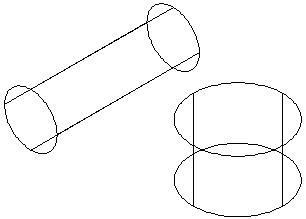
\includegraphics[scale=0.6]{chechukouduxiaojianmo2.png}}
\end{floatrow}
\end{figure}

\begin{lstlisting}
命令: cylinder
指定底面的中心点或 [三点(3P)/两点(2P)/切点、切点、半径(T)/椭圆(E)]:
指定底面半径或 [直径(D)]: 7
指定高度或 [两点(2P)/轴端点(A)]: 38
\end{lstlisting}

\item 构建切除圆柱体

接下来,我们需要在基础柱体完成切口的构建。观察主俯视图可知切口的形状是一圆柱面。因此需要构建一个与基础圆柱体中心轴线相垂直的,用于切除的圆柱体。为此需要先将视图切换为俯视图,以使$x-y$坐标平面与俯视图投影面平行。
\begin{lstlisting}
命令: -view 
输入选项 [?/删除(D)/正交(O)/恢复(R)/保存(S)/设置(E)/窗口(W)]:top
\end{lstlisting}

完成后再次将视图方向切换为西南等轴测。
\begin{lstlisting}
命令: -view 
输入选项 [?/删除(D)/正交(O)/恢复(R)/保存(S)/设置(E)/窗口(W)]:swiso 
\end{lstlisting}

接下来,再次调用圆柱体命令,在任意位置构建一个半径为R12,高度为14的圆柱体,结果如图\ref{fig:chechukouduxiaojianmo2}所示。之所以,取高度为14是因为基础圆柱体的直径是$\phi 14$,这样便能够保证完整地在基础圆柱体上切出想要的切口。
\begin{lstlisting}
命令: CYLINDER
指定底面的中心点或 [三点(3P)/两点(2P)/切点、切点、半径(T)/椭圆(E)]:
指定底面半径或 [直径(D)] <7.0000>: 12
指定高度或 [两点(2P)/轴端点(A)] <38.0000>: 14
\end{lstlisting}

\item 绘制辅助线

为方便进行实体定位,我们需要绘基础圆柱体和切除圆柱绘制用于定位的辅助线。在AutoCAD中可能用直线命令来完成辅助线的绘制,其调用方法有:

\begin{itemize}
\item 键盘输入line\index{line,直线} 或L。
\item 【绘图】$\rightarrow$【直线】
\item 【绘图】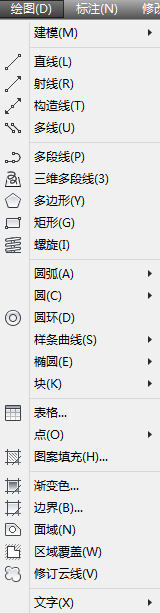
\includegraphics[scale=0.5]{drawtools.png}工具栏中的【直线】图标
\includegraphics[scale=0.5]{linetool.png}。
\end{itemize}

调用直线命令后需要指定两个具体的点,由于要绘制的辅助线是圆柱体的轴心线,因此需要指定圆柱体上顶圆和下底圆的圆位置作为直线的起点和终点。在此例中,我们并不知识具体的圆心坐标,因此需要应用AutoCAD中的捕捉功能来获取圆柱体圆心的位置。在AutoCAD中开启捕捉功能的方法有:

\begin{itemize}
	\item 键盘输入捕捉命令
	\item 
\includegraphics[scale=0.3]{keyctrl.png} + 鼠标右键,弹出图\ref{fig:buzhuomun}所示的对象捕捉菜单,选择相应的捕捉
	\item 【工具】$\rightarrow$【绘图设置】中的对象捕捉选项卡中设置相应的捕捉,如图\ref{fig:desettings}所示。
\end{itemize}

\begin{figure}[htbp]%
\centering
\begin{floatrow}[2]
\ffigbox{\caption{对象捕捉菜单}\label{fig:buzhuomun}}{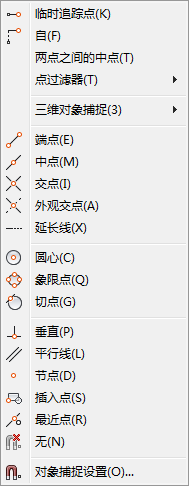
\includegraphics[scale=0.4]{buzhuomun.png}}
\ffigbox{\caption{对象捕捉设置}\label{fig:desettings}}{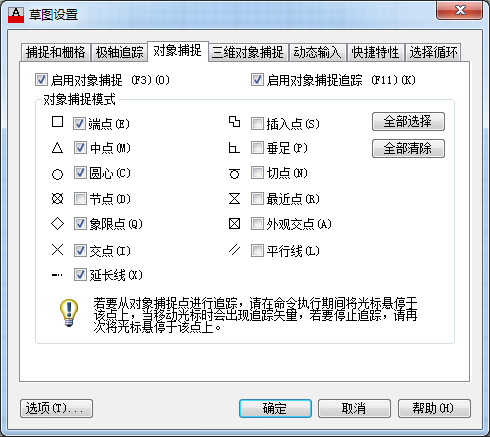
\includegraphics[scale=0.45]{desettings.png}}
\end{floatrow}
\end{figure}

捕捉设置完成后,即可用直线命令绘制基础圆柱体的中心轴线,首先用鼠标捕捉图\ref{fig:linedraw1}所示圆心作为直线的起点,捕捉图\ref{fig:linedraw2}所示圆心作为直线的终点,最终结果如图\ref{fig:chechukouduxiaojianmo3}所示。
\begin{lstlisting}
命令: line
指定第一个点:
指定下一点或 [放弃(U)]: 
指定下一点或 [放弃(U)]:
\end{lstlisting}

\begin{figure}[htbp]%
\centering
\subfloat[]{\label{fig:linedraw1}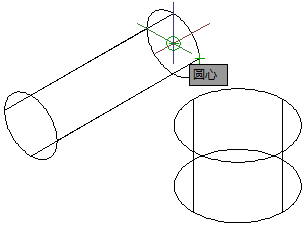
\includegraphics[width=0.4\textwidth]{linedraw1.png}}\hspace{20pt}
\subfloat[]{\label{fig:linedraw2}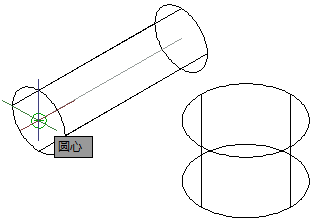
\includegraphics[width=0.4\textwidth]{linedraw2.png}}
\caption{直线绘制过程}
\end{figure}

用相同的方法绘制切除圆柱体的中心轴线,结果如图\ref{fig:chechukouduxiaojianmo4}所示。
\begin{lstlisting}
命令: line
指定第一个点:
指定下一点或 [放弃(U)]:
指定下一点或 [放弃(U)]:
\end{lstlisting}

\begin{figure}[htbp]%
\centering
\subfloat[]{\label{fig:chechukouduxiaojianmo3}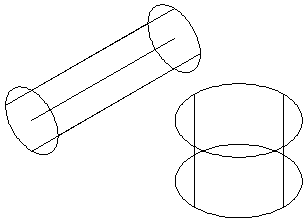
\includegraphics[width=0.4\textwidth]{chechukouduxiaojianmo3.png}}\hspace{20pt}
\subfloat[]{\label{fig:chechukouduxiaojianmo4}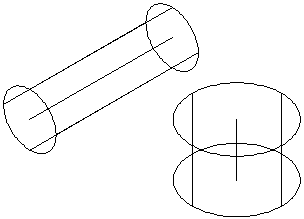
\includegraphics[width=0.4\textwidth]{chechukouduxiaojianmo4.png}}
\caption{辅助线绘制结果}
\end{figure}

\item 构建切口

从汽化器侧出口堵销零件的主视图中可知,切除圆柱体的轴心线与基础圆柱体的轴心线之间的垂直距离为17,为实现切除圆柱体轴线位置的准确定位,需要应用AutoCAD中的偏移命令将基础圆柱体的轴心辅助线向外偏移17。AutoCAD中调用偏移命令的方法有:

\begin{itemize}
\item 键盘输入offset\index{offset,偏移} 或o。
\item 【修改】$\rightarrow$【偏移】
\item 【修改】
\includegraphics[scale=0.5]{edittools.png}工具栏中的【偏移】图标
\includegraphics[scale=0.5]{offsettool.png}。
\end{itemize}

\begin{figure}[htbp]%
\centering
\subfloat[]{\label{fig:chechukouduxiaojianmo5}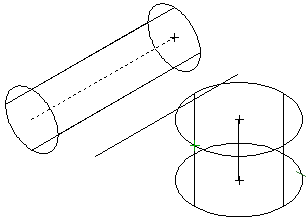
\includegraphics[width=0.4\textwidth]{chechukouduxiaojianmo5.png}}\hspace{20pt}
\subfloat[]{\label{fig:chechukouduxiaojianmo6}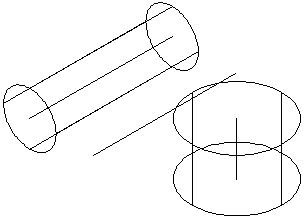
\includegraphics[width=0.4\textwidth]{chechukouduxiaojianmo6.png}}
\caption{偏移操作}
\end{figure}

调用偏移命令后,首先将偏移距离设置为17,接下来 选择基础圆柱体的轴心辅助线作为偏移对象;选择完成后,基础圆柱的轴心辅助线会以虚线的形式显示;然后来将鼠标偏向所选择对象的右侧,AutoCAD会显示偏移对象的位置,结果如图\ref{fig:chechukouduxiaojianmo5}所示。最后,单击鼠标左键确定偏移位置,最终结果如图\ref{fig:chechukouduxiaojianmo6}所示。
\begin{lstlisting}
命令: offset
当前设置: 删除源=否  图层=源  OFFSETGAPTYPE=0
指定偏移距离或 [通过(T)/删除(E)/图层(L)] <通过>:  17
选择要偏移的对象,或 [退出(E)/放弃(U)] <退出>:
指定要偏移的那一侧上的点,或 [退出(E)/多个(M)/放弃(U)] <退出>:
选择要偏移的对象,或 [退出(E)/放弃(U)] <退出>:
\end{lstlisting}

完成基础圆柱体的轴心辅助线偏移后,需要将切除圆柱体定位到偏移所得的辅助线上。此时,可以调用AutoCAD中的行移动命令来实现,其常用的调用方法有:

\begin{itemize}
	\item 键盘输入move\index{move,移动} 或m。
  \item 【修改】$\rightarrow$【移动】
  \item 【修改】
\includegraphics[scale=0.5]{edittools.png}工具栏中的【移动】图标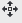
\includegraphics[scale=0.5]{movetool.png}。
\end{itemize}

\begin{figure}[htbp]%
\centering
\subfloat[]{\label{fig:moveselect1}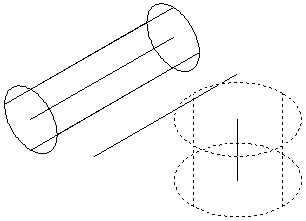
\includegraphics[width=0.2\textwidth]{moveselect1.png}}\hspace{10pt}
\subfloat[]{\label{fig:moveselect2}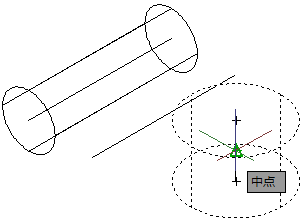
\includegraphics[width=0.2\textwidth]{moveselect2.png}}\hspace{10pt}
\subfloat[]{\label{fig:moveselect3}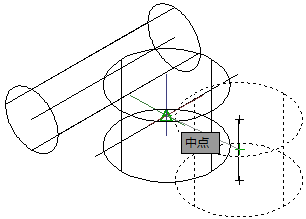
\includegraphics[width=0.2\textwidth]{moveselect3.png}}\hspace{10pt}
\subfloat[]{\label{fig:chechukouduxiaojianmo7}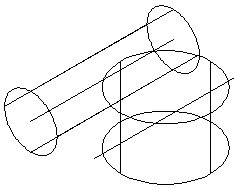
\includegraphics[width=0.2\textwidth]{chechukouduxiaojianmo7.png}}
\caption{移动操作}
\end{figure}

移动命令调用后,选择切除圆柱体作为移动对象,选择后会以虚线方式显示,结果如图\ref{fig:moveselect1}所示。接下来以图\ref{fig:moveselect2}所示方式捕捉切除圆柱体轴心辅助线的中点作为移动基点。最后以图\ref{fig:moveselect3}所示方式捕捉偏移辅助线的中点作为移动的目标点,即可完成切除圆柱体的准确定位,结果如图\ref{fig:chechukouduxiaojianmo7}所示。

\begin{lstlisting}
命令: move
选择对象: 找到 1 个
选择对象:
指定基点或 [位移(D)] <位移>:
指定第二个点或 <使用第一个点作为位移>:
\end{lstlisting}

完成切除圆柱体后,需要用切除圆柱从基础圆柱体中切出切口。在AutoCAD中实现这目的的命令是差集命令,其常用的调用方法有:

\begin{itemize}
\item 键盘输入SUBTRACT\index{subtract,差集}或SU。
\item 【修改】$\rightarrow$【实体编辑】$\rightarrow$【差集】
\item 【实体编辑】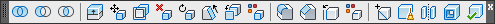
\includegraphics[scale=0.5]{solidedittools.png}【差集】图标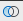
\includegraphics[scale=0.7]{subtracttool.png}。
\end{itemize}

调用差集命令后,以图\ref{fig:chechukouduxiaojianmo8}所示的基础圆柱体作为要从中切除的实体并确认,然后再选择图\ref{fig:chechukouduxiaojianmo9}所示的切除圆柱体作为要减去的实体并确认,最终结果如图\ref{fig:chechukouduxiaojianmo10}所示。

\begin{lstlisting}
命令: SUBTRACT
选择要从中减去的实体、曲面和面域...
选择对象: 找到 1 个
选择对象:  选择要减去的实体、曲面和面域...
\end{lstlisting}

\begin{figure}[htbp]%
\centering
\subfloat[]{\label{fig:chechukouduxiaojianmo8}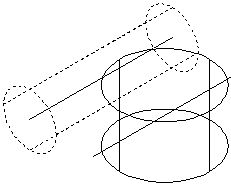
\includegraphics[width=0.3\textwidth]{chechukouduxiaojianmo8.png}}\hspace{10pt}
\subfloat[]{\label{fig:chechukouduxiaojianmo9}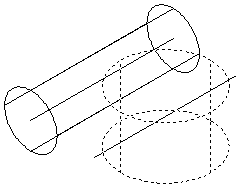
\includegraphics[width=0.3\textwidth]{chechukouduxiaojianmo9.png}}\hspace{10pt}
\subfloat[]{\label{fig:chechukouduxiaojianmo10}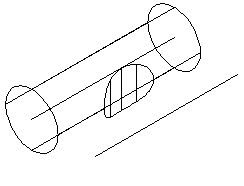
\includegraphics[width=0.3\textwidth]{chechukouduxiaojianmo10.png}}
\caption{差集操作}
\end{figure}

\item 删除辅助线

完成切口的建模后,辅助线的使命就已经结束了,因此需要将其从模型中删除。AutoCAD中实现图形对象删除的命令是删除,其调用方法有:

\begin{itemize}
\item 键盘输入eraset\index{erase,删除}或者delete\index{delete,删除} 或E。
\item 【修改】$\rightarrow$【删除】
\item 【修改】
\includegraphics[scale=0.5]{edittools.png}工具栏中的【删除】图标
\includegraphics[scale=0.5]{erase.png}。
\end{itemize}

\begin{figure}[htbp]%
\centering
\subfloat[]{\label{fig:chechukouduxiaojianmo11}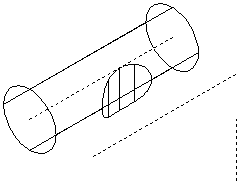
\includegraphics[width=0.4\textwidth]{chechukouduxiaojianmo11.png}}\hspace{20pt}
\subfloat[]{\label{fig:chechukouduxiaojianmo12}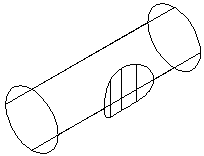
\includegraphics[width=0.3\textwidth]{chechukouduxiaojianmo12.png}}
\caption{删除操作}
\end{figure}

调用删除命令后,按图\ref{fig:chechukouduxiaojianmo11}方式选择三条辅助线作为删除对像并确认。删除辅助线后的结果如图\ref{fig:chechukouduxiaojianmo12}所示。

\begin{lstlisting}
命令: erase
选择对象: 找到 1 个
选择对象: 找到 1 个,总计 2 个
选择对象: 找到 1 个,总计 3 个
选择对象:
\end{lstlisting}

\item 构建倒角边

然后,应用AutoCAD中的倒角边命令完成两个倒角的构建,结果如图\ref{fig:chechukouduxiaojianmo13}所示。

\begin{lstlisting}
命令:  CHAMFEREDGE
距离 1 = 1.0000,距离 2 = 1.0000
选择一条边或 [环(L)/距离(D)]: d
指定距离 1 或 [表达式(E)] <1.0000>:
指定距离 2 或 [表达式(E)] <1.0000>:
选择一条边或 [环(L)/距离(D)]:
选择同一个面上的其他边或 [环(L)/距离(D)]:
选择同一个面上的其他边或 [环(L)/距离(D)]:
按 Enter 键接受倒角或 [距离(D)]:
\end{lstlisting}

\begin{figure}[htbp]%
\centering
\begin{floatrow}[2]
\ffigbox{\caption{倒角边}\label{fig:chechukouduxiaojianmo13}}{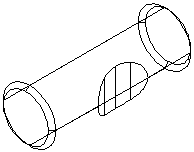
\includegraphics[scale=0.6]{chechukouduxiaojianmo13.png}}
\ffigbox{\caption{汽化器侧出口堵销模型}\label{fig:chechukouduxiaojianmo14}}{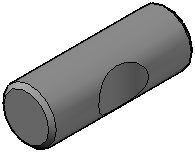
\includegraphics[scale=0.6]{chechukouduxiaojianmo14.png}}
\end{floatrow}
\end{figure}

\item 切换视觉样式

接下来,将模型空间的视觉样式切换为灰度,结果如图\ref{fig:chechukouduxiaojianmo14}所示。
\begin{lstlisting}
命令: vscurrent
输入选项 [二维线框(2)/线框(W)/隐藏(H)/真实(R)/概念(C)/着色(S)/带边缘着色(E)/灰度(G)/勾画(SK)/X 射线(X)/其他(O)] <二维线框>: g
\end{lstlisting}

\item 保存模型

最后,将建模完成的三维模型以“汽化器侧出口堵销.dwg”的名称予以保存。
\end{procedure}
\endinput